\usepackage{amsmath}

\usepackage{inputenc}
\usepackage{fvextra}

\usepackage{algpseudocode}
\usepackage{algorithmicx}
\usepackage{amsfonts}
\usepackage{amssymb}
\usepackage{amsthm}
\usepackage[spanish]{babel}
\usepackage{bm}
\usepackage{booktabs} % To thicken table lines
\usepackage{bussproofs}
\usepackage{caption}
\usepackage{csquotes}
\usepackage{colortbl}
\usepackage{dsfont}
\usepackage{environ}
\usepackage[shortlabels]{enumitem}
\usepackage{fancyhdr}
\usepackage{forest}
\usepackage{geometry}
\usepackage{graphicx}
\usepackage[hidelinks]{hyperref}
\usepackage{ifthen}
\usepackage{multicol}
\usepackage{multirow}
\usepackage{sidecap}
\usepackage{stmaryrd}
\usepackage{tabularx}
\usepackage{titling}
\usepackage{tikz}
\usepackage{xcolor}
\usepackage{wrapfig}
\usepackage{minted}

\usetikzlibrary{arrows}
\usetikzlibrary{arrows.meta}
\usetikzlibrary{automata}
\usetikzlibrary{calc}
\usetikzlibrary{fit}
\usetikzlibrary{matrix}
\usetikzlibrary{positioning}
\usetikzlibrary{shapes.geometric}
\usetikzlibrary{shapes.multipart}


\title{Teoría de Lenguajes}
\author{Gianfranco Zambonni}
%%%% CONFIGURACIONES %%%%

%% La coma de los reales es un punto
\decimalpoint{}

%%% Tamaño de pagina
%\geometry{
%	includeheadfoot,
%	left=2.54cm,
%	bottom=1cm,
%	top=1cm,
%	right=2.54cm
%}

%\stul{0.1cm}{0.2ex}

%% HEADER Y FOOTER
\pagestyle{fancy}

\fancyhf{}

\fancyhead[LO]{\rightmark} % \thesection\ 
\fancyhead[RO]{\small{\thetitle}}
\fancyfoot[CO]{\thepage}
\renewcommand{\headrulewidth}{0.5pt}
\renewcommand{\footrulewidth}{0.5pt}
\setlength{\headsep}{1cm}
\setlength{\headheight}{13.07225pt}

\renewcommand{\baselinestretch}{1.2}  % line spacing

%% Links en indice 
\hypersetup{
	linktoc=all,     %set to all if you want both sections and subsections linked
	linkcolor=blue,  %choose some color if you want links to stand out
}
\definecolor{darkgreen}{rgb}{0.0, 0.5, 0.0}

\newcommand{\red}[1]{{\color{red}#1}}
\newcommand{\blue}[1]{{\color{blue}#1}}
\newcommand{\green}[1]{{\color{darkgreen}#1}}

\newcommand{\deriva}{\overset{*}{\Rightarrow}}
\newcommand{\iffa}[1]{
  \underset{\text{#1}}{\iff}
}
\newcommand{\iffab}[2]{
  \underset{\text{#2}}{\iffa{#1}}
}

\newcommand{\thena}[1]{
  \underset{\text{#1}}{\implies}
}
\newcommand{\thenab}[2]{
  \underset{\text{#2}}{\thena{#1}}
}
\usetikzlibrary{shapes.multipart}

\tikzstyle{demoBox} = [
draw=blue!20, very thick,
rectangle split, rectangle split parts=2, rounded corners, inner xsep=0.5cm,
rectangle split part fill = {blue!20, blue!5}
]

\tikzstyle{demoPart} = [
draw=blue!20, very thick,
rounded corners, inner xsep=0.5cm,
fill = blue!5
]
%\newcommand{\qed}{\begin{flushright}
%		$\blacksquare$
%\end{flushright}}

\NewEnviron{demo}[1][]{%
  \begin{center}
    \begin{tikzpicture}
      \node [demoBox](box){%
        \textbf{\scriptsize
          DEMOSTRACIÓN}
        \nodepart{two}
        \begin{minipage}{#1}
          \vspace*{0.1cm}
          \BODY
        \end{minipage}
      };
    \end{tikzpicture}
  \end{center}
}

\NewEnviron{demoPart}[1][]{%
  \begin{center}
    \begin{tikzpicture}
      \node [demoPart](box){%
        \begin{minipage}{#1}
          \vspace*{0.1cm}
          \BODY
        \end{minipage}
      };
    \end{tikzpicture}
  \end{center}
}

\newtheorem{definicion}{Definición}[section]
\newtheorem{teorema}{Teorema}[section]
\newtheorem{corolario}{Corolario}[section]
\newtheorem{proposicion}{Proposición}[section]
\newtheorem{propiedad}{Propiedad}[section]
\newtheorem{lema}{Lema}[section]
\begin{document}

%%% TEOREMA 5.2 LOGICA - Conjunto consistentes (COMPLETAR HAY QUE PENSAR)
\maketitle
\tableofcontents
\newpage
\section{Introducción}
\subsection{Relaciones}
Dados dos conjuntos \(A\) y \(B\), se llama \textbf{relación} \(R\) de \(A\) en \(B\) a todo subconjutno de \(A\times B\). Notamos \(R:A\to B\).
\begin{itemize}
  \item \(aRb\) denota el hecho \((a,b)\in R\).
  \item Si \(A = B\) se dice que \(R\) es una relación sobre \(A\).
\end{itemize}

\noindent Una relación \(R: A\to A\) es
\begin{itemize}
  \item   \textbf{reflexiva} cuando \(\forall a\in A,~aRa\).
  \item \textbf{simétrica} cuando \(\forall a,b\in A,~aRb \implies bRa\).
  \item \textbf{transitiva} cuando \(a,b,c\in A,~aRb~\land~bRc\implies aRc\).
  \item es de \textbf{equivalencia} cuando es reflexiva, simétrica y transitiva. Este tipo de relaciones particiona a \(A\) en clases de equivalencia.
\end{itemize}

\subsubsection{Operaciones}
\paragraph{Composición de relaciones:} Si \(R:A\to B\) y \(S:B\to C\) son relaciones, entonces la composición de \(R\) y \(S\) es la relación \(S\circ R:A\to C\) definida por:
\[S\circ R = \{(a,c)~|~a\in A,~c\in C : \exists b\in B,~aRb~\land~bSc\}\].

\paragraph{Relación de identidad:} La relación de identidad sobre \(A\) es la relación \(id_A:A\to A\) definida por: \[I = \{(a,a)~|~a\in A\}\].
\begin{itemize}
  \item Es el elemento neutro de la composición de relaciones.
\end{itemize}

\paragraph{Relación de potencia:} Dado \(R: A\to A\) se define la relación de potencia \(R^k: A\to A\) como la composición de \(k\) copias de \(R\):
\[R^n = \left\{
  \begin{array}{ll}
    id_A           & \text{si } n = 0 \\
    R\circ R^{n-1} & \text{si } n > 0
  \end{array}
  \right.
\]

\paragraph{Clausura transitiva/positiva:} Dada una relación \(R:A\to A\) se define la clausura transitiva de \(R\) como la relación \(R^+\) definida por: \[R^+ = \bigcup_{n=1}^\infty R^n\]
\begin{enumerate}
  \item \(R\subseteq R^+\).
  \item \(R^+\) es transitiva
  \item Para toda relación \(G:A\to A\) tal que \(R\subseteq G \land G\) es transitiva, entonces \(R^+\subseteq G\), es decir \(R^+\) es la relación transitiva más pequeña que contiene a \(R\).
\end{enumerate}
\begin{demo}
  \begin{enumerate}
    \item[2)] Si \(a R^+ b\) entonces existe una secuencia de elementos \(a = a_0, a_1, \dots, a_n = b\) tales que \(a_i R a_{i+1}\) para todo \(i\in [0,n-1]\).

      Análogamente, como \(b R^+ c\) existe una secuencia de elementos \(b = b_0, b_1, \dots, b_m = c\) tales que \(b_i R b_{i+1}\) para todo \(i\in [0,m-1]\).

      Por lo tanto, \(a R^{n+m} c\), por lo que \(a R^+ c\).
    \item[3)] Si \(a R^+ b\) entonces existe una secuencia de elementos \(a = a_0, a_1, \dots, a_n = b\) tales que \(a_i R a_{i+1}\) para todo \(i\in [0,n-1]\).

      Como \(R\subseteq G\) entonces \(a_i G a_{i+1}\) para todo \(i\in [0,n-1]\). Como \(G\) es transitiva entonces la aplicación repetida de la transitividad nos lleva a que \(a_1 G a_n\), por lo que \(a G b\).
  \end{enumerate}
\end{demo}

\paragraph{Clausura transitiva reflexiva:} \[ R^* = R^+ \cup id_A = \bigcup_{n=0}^\infty R^n\]

Si \(A\) es un conjunto finito, entonces todas las relaciones \(R:A\to A\) son finitas.

Si \(R\) es reflexiva, entonces \(R^* = R^+\).

\subsection{Alfabetos}
Un alfabeto es un conjunto finito de símbolos.

\paragraph{Cadena:} Una cadena sobre un alfabeto \(\Sigma\) es una secuencia finita de símbolos de \(\Sigma\). Los símbolos son notados respetando el orden de la secuencia.

\subsubsection{Operaciones}
\paragraph{Concatenación:} Es una operación entre un símbolo del alfabeto \(\Sigma\) y una cadena sobre dicho alfabeto:
\[ \circ : \Sigma\times\{\text{cadenas sobre }\Sigma\}\to\{\text{cadenas de }\Sigma\}\]
\begin{itemize}
  \item La cadena nula \(\lambda\) es el elemento neutro de la concatenación.
\end{itemize}

\paragraph{Clausura de Kleene de \(\Sigma\): \(\Sigma^*\)}
\begin{itemize}
  \item \(\lambda\in\Sigma^*\)
  \item \(a\in\Sigma \land^*\implies \forall~\alpha\in\Sigma,~a\circ\alpha\in\Sigma^*\)
\end{itemize}

\paragraph{Clausura positiva de \(\Sigma\):} \(\Sigma^+ = \Sigma^*\setminus\{\lambda\}\)

\subsection{Lenguajes}
Un lenguaje es un conjunto de cadenas sobre un alfabeto \(\Sigma\).

\subsubsection{Operaciones}
\paragraph{Concatenación de lenguajes:} Si \(L_1\) y \(L_2\) son lenguajes definidos sobre los alfabetos \(\Sigma_1\) y \(\Sigma_2\) respectivamente, entonces la concatenación de \(L_1\) y \(L_2\) es el lenguaje \(L_1L_2\) definido por:
\[ L_1L_2 = \{ \alpha\beta~|~\alpha\in L_1,~\beta\in L_2\}\]
definido sobre el alfabeto \( \Sigma_1\cup\Sigma_2\).

\paragraph*{Clausura de Kleene \(L^*\):} Se define por:
\begin{align*}
  L^0 & = \{\lambda\}                 \\
  L^n & = LL^{n-1} \text{ para } n>=1 \\
  L^* & = \bigcup_{n=0}^\infty L^n
\end{align*}
\paragraph{Clausura positiva \(L^+\):} \(L^+ = \bigcup_{n=1}^\infty L^n\)
\begin{itemize}
  \item \(L^+ = LL^*\)
  \item \(L^* = L^+\cup\{\lambda\}\)
  \item Si \(L\) es un lenguaje definido sobre \(\Sigma\) entonces \(L\subseteq\Sigma^*\)
\end{itemize}
\subsection{Gramáticas}
Una gramática es una 4-tupla \((V_N,V_T,P,S)\) donde:
\begin{itemize}
  \item \(V_N\) es un conjunto finito de símbolos no terminales.
  \item \(V_T\) es un conjunto finito de símbolos terminales.
  \item \(P\) es un conjunto finito de reglas de producción: Son pares ordenados \(\alpha,\beta\) donde \(\alpha\in(V_N\cup V_T)^*V_N(V_N\cup V_T)^*\) y \(\beta\in(V_N\cup V_T)^*\).

        Las notamos como \(\alpha\to\beta\).
  \item \(S\in V_N\) es el símbolo inicial.
\end{itemize}

\paragraph{Forma setencial de una grámatica:} Se llama forma sentencial a una derivación de la misma (es decir, una cadena formada por símbolos de \(V_N\cup V_T\) que sea el resultado de una derivación a partir de símbolos iniciales):
\begin{itemize}
  \item \(S\) es una forma setencial de \(G\)
  \item Si \(\alpha\beta\gamma\) es una forma setencial de \(G\) y \(\beta\to\delta\in P\) entonces \(\alpha\delta\gamma\) es una forma setencial de \(G\).
\end{itemize}

\paragraph{Derivación directa en \(G\):} Si \(\alpha\beta\lambda\in(V_N\cup V_T)^*\) y \(\beta\to\delta\in P\) entonces \(\alpha\delta\lambda\) es una derivación directa de \(G\) de \(\alpha\beta\lambda\) y se denota como \(\alpha\beta\lambda\underset{G}{\implies}\alpha\delta\lambda\).

Denotaremos con \(\overset{+}{\underset{G}{\implies}}\) y \(\overset{*}{\underset{G}{\implies}}\) a la clausura positiva y la clausura transitiva y reflexiva de \(\underset{G}{\implies}\), respectivamente.

Además, \(\overset{k}{\underset{G}{\implies}}\) será la potencia \(k\)-ésima de \(\underset{G}{\implies}\).

\paragraph{Lenguaje de una grámatica \(\mathcal{L}(G)\):} Es el conjunto de todas las cadenas de símbolos terminales que son formas setenciales de \(G\).

\[ \mathcal{L}(G) = \{ \alpha\in V_T^*:~S\overset{+}{\underset{G}{\implies}}\alpha\}\]

\subsubsection{Clasificación de grámaticas (Chomsky)}
\paragraph{Gramáticas regulares (tipo 3):} Son aquellas gramáticas que cumplen alguna de las siguientes condiciones:
\begin{itemize}
  \item Todas sus producciones son de la forma \(A\to aB\) ó \(A\to a\) ó \(A\to\lambda\) donde \(A,B\in V_N\) y \(a\in V_T\). En este caso se dice que es una gramática lineal a derecha.
  \item Todas sus producciones son de la forma \(A\to Ba\) ó \(A\to a\) ó \(A\to\lambda\) donde \(A,B\in V_N\) y \(a\in V_T\). En este caso se dice que es una gramática lineal a izquierda.
\end{itemize}

\paragraph{Gramáticas libres de contexto (tipo 2):} Son aquellas gramáticas en las que cada producción es de la forma \(A\to\alpha\) donde \(A\in V_N\) y \(\alpha\in(V_N\cup V_T)^*\).

De la definición anterior puede inferirse que toda grámatica regular es libre de contexto.

\paragraph{Gramáticas sensibles al contexto (tipo 1):} Son aquellas gramáticas en las que cada producción es de la forma \(\alpha\to\beta\) donde \(\alpha,\beta\in(V_N\cup V_T)^*\) y \(|\alpha|\leq |\beta|\).

Se puede inferir que toda gramática independiente del contexto que no posea regla borradoraas (es decir, que no posea producciones de la forma \(A\to\lambda\)) es sensible al contexto.

\paragraph{Gramáticas sin restricciones (tipo 0):} Son aquellas gramáticas que no poseen ninguna restricción como las anteriores.

El conjunto de las grámaticas tipo 0 es el conjunto de todas las grámaticas.

\paragraph{Definición:} Un lenguaje generado por una grámatica tipo \(t\) es llamado \textbf{lenguaje tipo \(t\)}.

\newpage
\section{Autómatas finitos}
\subsection{Autómatas finitos deterministicos (AFD)}
Un autómata finito determinista es una 5-tupla \(\mathcal{M}=\langle Q,\Sigma,\delta,q_0,F\rangle\) donde:
\begin{itemize}
  \item \(Q\) es un conjunto finito de estados.
  \item \(\Sigma\) es un conjunto finito de símbolos de entrada.
  \item \(\delta:Q\times\Sigma\to Q\) es una función de transición.
  \item \(q_0\in Q\) es el estado inicial.
  \item \(F\subseteq Q\) es el conjunto de estados finales.
\end{itemize}

\paragraph{Función de transición generalizada \(\hat{\delta}\):} La función de transición \(\delta\) está definida para que tome como parámetro un único símbolo de \(Sigma\). Se puede extender para que tomé como parámetro una cadena de símbolos de \(Sigma\):
\[ \hat{\delta} : Q\times\Sigma^*\to Q\]

se define de manera recursica como:
\begin{itemize}
  \item \(\hat{\delta}(q,\lambda)=q\)
  \item \(\hat{\delta}(q,\beta a)=\delta(\hat{\delta}(q,\beta),a)\) con \(\beta\in\Sigma^*\) y \(a\in\Sigma\)
\end{itemize}

\paragraph{Cadena aceptada por un AFD:} Una cadena \(\beta\in\Sigma^*\) es aceptada por un AFD \(\mathcal{M} = \langle Q, \Sigma, \delta, q_0, F\rangle\) si y solo si \(\hat{\delta}(q_0,\beta)\in F\).

\paragraph{Lenguaje aceptado por un AFD:} El lenguaje aceptado por un AFD \(\mathcal{M} = \langle Q, \Sigma, \delta, q_0, F\rangle\) es el conjunto de todas las cadenas \(\beta\in\Sigma^*\) que son aceptadas por \(\mathcal{M}\):
\[ L(\mathcal{M}) = \{ \beta\in\Sigma^*:~\hat{\delta}(q_0,\beta)\in F\}\]

\subsection{Autómatas finitos no deterministas (AFND)}
Un autómata finito no determinista es una 5-tupla \(\mathcal{M}=\langle Q,\Sigma,\delta,q_0,F\rangle\) donde:
\begin{itemize}
  \item \(Q\) es un conjunto finito de estados.
  \item \(\Sigma\) es un conjunto finito de símbolos de entrada.
  \item \red{\(\delta:Q\times\Sigma\to \mathcal{P}(Q)\)} es una función de transición.

        A diferencia de los AFD, la función \(\delta\) devuelve un conjunto de estados en lugar de un solo estado.
  \item \(q_0\in Q\) es el estado inicial.
  \item \(F\subseteq Q\) es el conjunto de estados finales.
\end{itemize}

\paragraph{Función de transición generalizada \(\hat{\delta}\):} Primero vamos a definir \(\delta_P : \mathcal{P}(Q)\times\Sigma\to\mathcal{P}(Q)\) de la siguiente manera:
\[ \delta_P(P,a) = \underset{p\in P}{\bigcup}\delta(p,a)\]

La función \(\hat{\delta} : Q\times\Sigma^*\to \mathcal{P}(Q)\) se define de manera recursiva como:
\begin{itemize}
  \item \(\hat{\delta}(q,\lambda)=\{q\}\)
  \item \(\hat{\delta}(q,\beta a)= \{ p:~\exists r\in\hat{\delta}(q,\beta)\) tal que \(p \in \delta(r, a)\} = \delta_P(\hat{\delta}(q, \beta), a)\) con \(\beta\in\Sigma^*\) y \(a\in\Sigma\)
\end{itemize}

Para generalizar a un más podemos definir \(\hat{\delta}_P : \mathcal{P}(Q)\times\Sigma^*\to\mathcal{P}(Q)\) de la siguiente manera:
\[ \hat{\delta}_P(P,\beta) = \underset{q\in P}{\bigcup}\hat{\delta}(q,\beta)\]

\paragraph{Cadena aceptada por un AFND:} Una cadena \(\beta\in\Sigma^*\) es aceptada por un AFND \(\mathcal{M} = \langle Q, \Sigma, \delta, q_0, F\rangle\) si y solo si \(\hat{\delta}(q_0,\beta)\cap F \neq \emptyset\). Es decir, si alguno de los estados alcanzados por \(\hat{\delta}(q_0,\beta)\) es un estado final.

\paragraph{Lenguaje aceptado por un AFND:} El lenguaje aceptado por un AFND \(\mathcal{M} = \langle Q, \Sigma, \delta, q_0, F\rangle\) es el conjunto de todas las cadenas \(\beta\in\Sigma^*\) que son aceptadas por \(\mathcal{M}\):
\[ L(\mathcal{M}) = \{ \beta\in\Sigma^*:~\hat{\delta}(q_0,\beta)\cap F \neq \emptyset\}\]

\subsubsection{Equivalencia entre AFD y AFND}
Es trivial ver que para todo AFD existe un AFND que acepte el mismo lenguaje.

\begin{teorema}
  Dado una AFND \(\mathcal{M} = \langle Q, \Sigma, \delta, q_0, F\rangle\), existe un AFD \(\mathcal{M}' = \langle Q', \Sigma, \delta', q_0', F'\rangle\) tal que \(L(\mathcal{M}) = L(\mathcal{M}')\).
\end{teorema}
Vamos a demostrar este teorema construyendo una AFD \(\mathcal{M}'\) a partir de \(\mathcal{M}\). Una vez constuido deberemos demostrar que \(\mathcal{M}'\) acepta el mismo lenguaje que \(\mathcal{M}\).

\paragraph{Construcción de \(\mathcal{M}'\):}
\begin{itemize}
  \item \(Q'\) será el conjunto de partes \(\mathcal{P}(Q)\) que contenga a todos los posibles conjuntos de estados de \(\mathcal{M}\). Vamos a denotar cada estado \(s\in Q'\) con etiquetas del estilo \([q_1,\dots, q_k]\) donde \(q_1,\dots,q_k\in Q\). Entonces:
        \[ Q' = \mathcal{P}(Q)\]
  \item \(\delta'([q_1,\dots, q_k],a) = [p_1, \dots, p_m] \iff \delta_P(\{q_1,\dots,q_k\},a) = \{p_1,\dots,p_m\}\)
  \item \(q_0' = [q_0]\)
  \item \(F' = \{ [q_1,\dots, q_n]\in Q' : \{q_1,\dots,q_n\}\cap F \neq \emptyset\}\)
\end{itemize}

\paragraph{Equivalencia de funciónes de transición generalizadas:} Antes de demostrar que ambos automátas aceptan el mismo lenguaje, vamos a demostrar que las funciones de transición generalizadas de ambos automátas son equivalentes cuando las llamamos con el estado inicial como primer parámetro. Es decir, queremos ver que \(\hat{\delta}'(q_0',\beta) = [p_1,\dots,p_k] \iff \hat{\delta}(q_0,\beta) = \{p_1,\dots, p_k\}\).

Lo vamos a hacer por inducción. Recordemos que \(q_0' = [q_0]\):
\begin{itemize}
  \item Caso base: \(\beta = \lambda\):
        \begin{itemize}
          \item \(\hat{\delta}'([q_0],\lambda) = [q_0]\) por definición de \(\hat{\delta}'\).
          \item \(\hat{\delta}(q_0,\lambda) = \{q_0\}\) por definición de \(\hat{\delta}\).
        \end{itemize}
        Luego \(\hat{\delta}'([q_0],\lambda) = [q_0] \iff \hat{\delta}(q_0,\lambda) = \{q_0\}\).

  \item Caso inductivo: \(\beta \implies \beta a\): Por hipotesis inductiva tenemos que \[\hat{\delta}'(q_0',\beta) = [r_1,\dots,r_m] \iff \hat{\delta}(q_0,\beta) = \{r_1,\dots, r_m\}\]
        Queremos ver que \(\hat{\delta}'(q_0',\beta a) = [p_1,\dots,p_m] \iff \hat{\delta}(q_0,\beta a) = \{p_1,\dots, p_m\}\)
        \begin{align*}
           & \hat{\delta}'(q_0',\beta a) = [p_1,\dots,p_k]  \underset{\text{def.}}{\iff} \delta'(\hat{\delta}'(q_0',\beta),a) = [p_1,\dots,p_k]                                           \\
           & \underset{\text{def.}}{\iff} \exists [r_1,\dots,r_m]\in Q' \text{ tal que } \delta'(q_0',\beta) = [r_1,\dots,r_m] \land \delta'([r_1,\dots,r_m],a) = [p_1,\dots,p_k]         \\
           & \underset{H.I.}{\iff} \exists \{   r_1,\dots,r_m\}\in Q \text{ tal que } \hat{\delta}(q_0,\beta) = \{r_1,\dots,r_m\} \land \delta_P(\{r_1,\dots,r_m\},a) = \{p_1,\dots,p_k\} \\
           & \underset{\text{def.}}{\iff} \delta_P(\hat{\delta}(q_0,\beta),a) = \{p_1,\dots,p_k\} \underset{\text{def.}}{\iff} \hat{\delta}(q_0,\beta a) = \{p_1,\dots,p_k\}
        \end{align*}
\end{itemize}

\paragraph{Demostración de la equivalencia:} Ahora que hemos demostrado que las funciones de transición generalizadas de ambos automátas son equivalentes, vamos a demostrar que ambos automátas aceptan el mismo lenguaje:

\begin{align*}
  \beta \in \mathcal{L}(\mathcal{M}) & \underset{\text{def.}}{\iff} \hat\delta(q_0, \beta) = \{q_1,\dots, q_n\}\land\{q_1,\dots,q_n\}\cap F \neq \emptyset                                                                              \\
                                     & \iff \underbrace{\hat\delta(q_0', \beta) = [q_1,\dots, q_n]}_{\text{\scriptsize por equivalencia de generalizaciones}} \land~~~~~~\underbrace{[q_1,\dots,q_n]\in F'}_{\text{\scriptsize def.}F'} \\
                                     & \underset{def.}{\iff} x\in\mathcal{L}(M')
\end{align*}

\subsection{Autómatas finitos no deterministico con transiciones  \texorpdfstring{\(\lambda\)}{lambda}}
\label{sec:afd-lambda}
Un autómata finito no determinista con transiciones \(\lambda\) es un autómata finito no determinista que tiene transiciones \(\lambda\). Estas transacciones nos permiten ir de un estado a otro sin consumir ningún símbolo de entrada.

Los definimos con una 5-upla \((Q,\Sigma,\delta,q_0,F)\) donde:
\begin{itemize}
  \item \(Q\) es un conjunto finito de estados.
  \item \(\Sigma\) es un conjunto finito de símbolos de entrada.
  \item \red{\(\delta : Q \times (\Sigma \cup \{\lambda\}) \to \mathcal{P}(Q)\)} es una función de transición.
  \item \(q_0 \in Q\) es el estado inicial.
  \item \(F \subseteq Q\) es el conjunto de estados finales.
\end{itemize}

\paragraph{Clausura \(\lambda\) de un estado \(q\):} Se denota \(Cl_\lambda(q)\) es el conjunto de estados que se pueden alcanzar desde \(q\) siguiendo solo transiciones \(\lambda\). Es decir, \[Cl_\lambda(q) = \delta(q,\lambda)\]

Además \(q\in Cl_\lambda(q)\).

\paragraph{Clausura \(\lambda\) de un conjunto de estados \(P\):} \[Cl_{P\lambda}(P) = \bigcup_{p\in P} Cl_\lambda(p)\]
\paragraph{Generalización de la función de transición:}
Podemos extender \(\delta\) a conjunto de estados:
\begin{align*}
   & \delta_P: \mathcal{P}(Q) \times (\Sigma \cup \{\lambda\}) \to \mathcal{P}(Q) \\
   & \delta_P(P,a) = \underset{p\in P}{\bigcup} \delta(p,a)
\end{align*}

Entonces podemos definir:

\begin{align*}
   & \hat\delta: Q \times \Sigma^* \to \mathcal{P}(Q)                                                                                                                                                             \\
   & \hat\delta(q_0,\lambda) = Cl_\lambda(q_0)                                                                                                                                                                    \\
   & \hat\delta(q_0, \beta a) = Cl_{P\lambda}\left(\delta_P(\hat\delta(q_0,\beta), a)\right) = Cl_{P\lambda}\left(\left\{ p: \exists q\in \hat\delta(q_0,\beta) \text{ tal que } p\in \delta(q,a) \right\}\right)
\end{align*}

Tambien extendemos \(\hat\delta\) a conjuntos de estados:
\begin{align*}
   & \hat\delta_P: \mathcal{P}(Q) \times \Sigma^* \to \mathcal{P}(Q)  \\
   & \hat\delta_P(P,\beta a) = \bigcup_{p\in P} \hat\delta(p,\beta a)
\end{align*}

\paragraph{Cadena aceptada por un AFND-\(\lambda\):} Una cadena \(\beta\) es aceptada por un AFND-\(\lambda\) \(M =\langle Q,\Sigma,\delta,q_0,F\rangle\) si y solo si \(\hat\delta(q_0,\beta)\cap F \neq \emptyset\).

\paragraph{Lenguaje aceptado por un AFND-\(\lambda\):} El lenguaje aceptado por un AFND-\(\lambda\) \(M =\langle Q,\Sigma,\delta,q_0,F\rangle\) es el conjunto de todas las cadenas aceptadas por \(M\):
\[\mathcal{L}(M) = \{\beta \in \Sigma^* : \hat\delta(q_0,\beta)\cap F \neq \emptyset\}\]

\subsubsection{Equivalencia entre AFND y AFND-\texorpdfstring{\(\lambda\)}{lambda}}
\label{sec:afd-afd-lambda}
Dado un AFND-\(\lambda\) \(M =\langle Q,\Sigma,\delta,q_0,F\rangle\) podemos construir un AFND \(M' =\langle Q,\Sigma,\delta',q_0,F'\rangle\) tal que \(M\) acepte el mismo lenguaje que \(M'\).

\paragraph{Construcción de M':} Notemos que ambos autómatas tiene el mismo conjunto de estados \(Q\), el mismo conjunto de símbolos de entrada \(\Sigma\) y el mismo estado inicial \(q_0\). Por lo que solo debemos definir \(\delta'\) y \(F'\).
\begin{itemize}
  \item \(\delta'(q,a) = \hat\delta(q, a) = Cl_{P\lambda}\left(\delta_P(\hat\delta(q,\lambda), a)\right)\)
  \item \(
        F' = \begin{cases}
          F\cup\{q_0\} & \text{si } Cl_{P\lambda}(q_0)\cap F \neq \emptyset \\
          F            & \text{si no}
        \end{cases}\)
\end{itemize}

\paragraph{Equivalencia de funciones de transición generalizada:} Vamos a demostrar por inducción que \(\hat\delta'(q_0,\beta) = \hat\delta(q_0,\beta)\) para todo \(|\beta|\geq 1\):
\begin{itemize}
  \item Caso base: \(|\beta|=1\). Sea \(\beta = a\), entonces \(\hat\delta'(q_0,\beta) = \hat\delta'(q_0, a) = \hat\delta(q_0, a)\) por como definimos \(\delta'\).
  \item Caso inductivo: Supongamos que \(\hat\delta'(q_0,\beta) = \hat\delta(q_0,\beta)\) para todo \(|\beta|\leq n\). Sea \(\omega = \beta a\). Entonces:
        \begin{align*}
          \hat\delta'(q_0,\omega) & = \hat\delta'(q_0,\beta a) \underset{\text{def.}}{=} \delta'_P(\hat\delta'(q_0,\beta), a) \underset{\text{H.I}}{=} \delta'_P  (\hat\delta(q_0,\beta), a)\hspace*{1cm}(1) \\
        \end{align*}
        Por otro lado, dado \(P \subseteq Q\) tenemos que:
        \begin{align*}
          \delta_P'(P, a) & \underset{\text{def.}}{=} \bigcup_{p\in P} \delta'(p, a) \underset{\text{construcción de } M'}{=} \bigcup_{p\in P} \hat\delta(p, a)\underset{\text{def}}{=} \hat\delta_P(P,a)
        \end{align*}
        Entonces, remplazando en (1) el último término con este resultado, nos queda:
        \begin{align*}
          \delta'_P(\hat\delta(q_0,\beta), a) & = \hat\delta_P(\hat\delta(q_0,\beta), a) \underset{\text{def.}}{=} \hat\delta(q_0,\beta a) \underset{\text{def.}}{=} \hat\delta(q_0,\omega)
        \end{align*}
\end{itemize}

\paragraph{Demostración de equivalencia:} Veamos ahora que \(M\) acepta el mismo lenguaje que \(M'\), vamos a separar la demostración en dos casos: \(\beta=\lambda\) y \(\beta \neq \lambda\).
\begin{itemize}
  \item \(\beta=\lambda\)
        \begin{itemize}
          \item \(\lambda\in\mathcal{L}(M) \implies \lambda\in\mathcal{L}(M')\)
                \begin{align*}
                   & \lambda\in \mathcal{L}(M)  \underset{def.}{\implies} \hat\delta(q_0,\lambda)\cap F \neq \emptyset \underset{def.}{\implies} Cl_{\lambda}(q_0)\cap F \neq \emptyset \\
                   & \underset{\text{por construcción }M'}{\implies} q_0\in F' \underset{def.}{\implies} \lambda\in \mathcal{L}(M')
                \end{align*}
          \item \(\lambda\in\mathcal{L}(M') \implies \lambda\in\mathcal{L}(M)\).
                \begin{align*}
                   & \lambda\in \mathcal{L}(M')  \underset{\text{def.}}{\implies} q_0\in F' \underset{\text{construcción } M'}{\implies} q_0\in F \lor Cl_\lambda(q_0)\cap F \neq\emptyset \\
                \end{align*}
                Como \(q_0\in F \implies Cl_\lambda(q_0)\cap F \neq\emptyset\), entonces:
                \begin{align*}
                  q_0\in F \lor Cl_\lambda(q_0)\cap F \neq\emptyset \implies Cl_\lambda(q_0)\cap F \neq\emptyset \underset{\text{def.}}{\implies} \lambda\in \mathcal{L}(M)
                \end{align*}
        \end{itemize}
  \item \(\beta \neq \lambda\)
        \begin{itemize}
          \item \(\beta\in\mathcal{L}(M) \implies \beta\in\mathcal{L}(M')\)
                \begin{align*}
                   & \beta\in \mathcal{L}(M) \underset{\text{def.}}{\implies} \hat\delta(q_0,\beta)\cap F \neq \emptyset \underset{\text{por equivalencia transiciones}}{\implies} \delta'(q_0,\beta)\cap F \\
                   & \underset{\text{construcción } M'}{\implies} \delta'(q_0,\beta)\cap F' \neq \emptyset \underset{\text{def.}}{\implies} \beta\in \mathcal{L}(M')
                \end{align*}
          \item \(\beta\in\mathcal{L}(M') \implies \beta\in\mathcal{L}(M)\)
                \begin{align*}
                   & \beta\in \mathcal{L}(M') \underset{\text{def.}}{\implies} \delta'(q_0,\beta)\cap F' \neq \emptyset \underset{\text{equiv. transiciones}}{\implies} \hat\delta(q_0,\beta)\cap F' \neq \emptyset \\
                   & \underset{\text{constr.} M'}{\implies} \hat\delta(q_0,\beta)\cap F \neq \emptyset \lor \hat\delta(q_0,\beta)\cap(F\cup\{q_0\}) \neq \emptyset
                \end{align*}
                Si vale la primera parte de la última expresión \(\delta(q_0,\beta)\cap F \neq \emptyset\) entonces \(\beta\in \mathcal{L}(M)\) por definición.

                Veamos que pasa si vale \(\hat\delta(q_0,\beta)\cap(F\cup\{q_0\}) \neq \emptyset\):
                \begin{align*}
                  \hat\delta(q_0,\beta)\cap(F\cup\{q_0\}) \neq \emptyset \implies \hat\delta(q_0,\beta)\cap F \neq \emptyset \lor \hat\delta(q_0,\beta)\cap\{q_0\} \neq \emptyset
                \end{align*}

                La primer parte es lo mismo que arriba, analizemos la segunda:
                \begin{align*}
                  \hat\delta(q_0,\beta)\cap\{q_0\} \neq \emptyset \implies Cl_\lambda(q_0)\cap F \neq \emptyset \implies \lambda\in \mathcal{L}(M)
                \end{align*}
        \end{itemize}
\end{itemize}
Queda demostrada la equivalencia de lenguajes.

\newpage
\section{Expresiones regulares}
Una expresión regular es una expresión que describe un lenguaje de forma compacta y sencilla:

\begin{itemize}
  \item \(\varnothing\) es una expresión regular que describe el lenguaje vacío \(\emptyset\).
  \item \(\lambda\) es una expresión regular que describe el lenguaje unitario \(\{\lambda\}\).
  \item Para cada \(a\in\sigma\), \(a\) es una expresión regular que describe el lenguaje \(\{a\}\).
  \item Si \(r\) y \(s\) son dos expresiones que denotan los lenguajes \(R\) y \(S\) entonces:
        \begin{itemize}
          \item \(r|s\) ó \(r+s\) es una expresión regular que describe el lenguaje \(R\cup S\).
          \item \(rs\) es una expresión regular que describe el lenguaje \(RS\).
          \item \(r^*\) es una expresión regular que describe el lenguaje \(R^*\).
          \item \(r^+\) es una expresión regular que describe el lenguaje \(R^+\).
        \end{itemize}
\end{itemize}

\paragraph{Expresiones regulares recursivas:} Si \(r=\alpha r + \beta\), entonces \(r = \alpha^* \beta\). Además, si \(\alpha^* = \alpha^+\), entonces \(r = \alpha^*(\beta + \gamma)\) para culquier expresión regular \(\gamma\).

\subsection{Expresiones regulares a AFND-\texorpdfstring{\(\lambda\)}{Lambda}}
Dada una expresión regular \(r\), existe una AFND-\(\lambda\) \(M\) con un solo estado final y sin trancisiones a partir del mismo tal que \(\mathcal{L}(M) = \mathcal{L}(r)\).

Vamosa a demostrar por inducción sobre los operadores de las expresiones regulares.

\subsubsection{Casos base}
\begin{figure}[H]
  \begin{center}
    \caption*{\(r=\varnothing\)}
    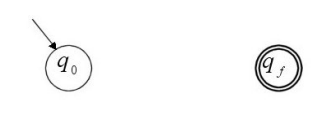
\includegraphics[scale=0.5]{imagenes/nothing}
  \end{center}
\end{figure}
\begin{figure}[H]
  \begin{center}
    \caption*{\(r=\lambda\)}
    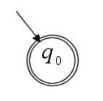
\includegraphics[scale=0.5]{imagenes/lambda}
  \end{center}
\end{figure}
\begin{figure}[H]
  \begin{center}
    \caption*{\(r=a\)}
    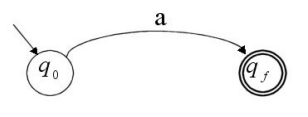
\includegraphics[scale=0.5]{imagenes/a}
  \end{center}
\end{figure}

\subsubsection{Pasos inductivos}
Sean \(r_1\) y \(r_2\) dos expresiones regulares. Supongamos que existen AFND-\(\lambda\) \\ \(M_1=\langle Q_1, \Sigma_1, \delta_1, q_1, \{f_1\}\rangle\) y \(M_2 =\langle Q_2, \Sigma_2, \delta_2, q_2, \{f_\}\rangle\) tal que \(\mathcal{L}(M_1) = \mathcal{L}(r_1)\) y \(\mathcal{L}(M_2) = \mathcal{L}(r_2)\). Vamos a armar a partir de estos autómata uno nuevo que acepte los lenguajes generados por las expresiones \(r_1|r_2\), \(r_1r_2\), \(r_1^*\) y \(r^+\).

\paragraph{\(\bm{r_1|r_2}\):} Podemos construir un automata \(M_0=\langle Q_0, \Sigma_0, \delta_0, q_0, \{f_0\}\rangle\) tal que \(\mathcal{L}(M_0) = \mathcal{L}(r_1|r_2)\) de la siguiente forma:
\begin{itemize}
  \item \(Q_0 = Q_1 \cup Q_2 \cup \{q_0, f_0\}\)
  \item \(\Sigma_0 = \Sigma_1 \cup \Sigma_2\)
  \item \(\delta_0: Q_0 \times \Sigma_0 \rightarrow \mathcal{P}(Q_0)\)
        \begin{itemize}
          \item[] \(\delta(q_0, \lambda) = \{q_1, q_2\}\)
          \item[] \(\delta(q, a) = \delta_1(q, a)\) para \(q\in Q_1-\{f_1\}\) y \(a\in \Sigma_1\cup\{\lambda\}\)
          \item[] \(\delta(q, a) = \delta_2(q, a)\) para \(q\in Q_2-\{f_2\}\) y \(a\in \Sigma_2\cup\{\lambda\}\)
          \item[] \(d(f_1,\lambda) = d(f_2,\lambda) = \{f_0\}\)
        \end{itemize}
\end{itemize}
\begin{figure}[H]
  \begin{center}
    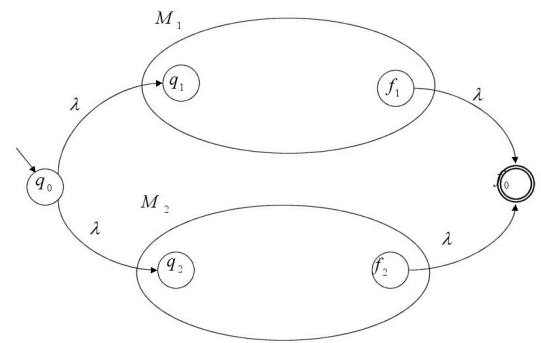
\includegraphics[scale=0.5]{imagenes/union}
  \end{center}
\end{figure}

\paragraph{\(\bm{r_1r_2}\):} \(M_0=\langle Q_0, \Sigma_0, \delta_0, q_1, \{f_2\}\rangle\):
\begin{itemize}
  \item \(Q_0 = Q_1 \cup Q_2\)
  \item \(\Sigma_0 = \Sigma_1 \cup \Sigma_2\)
  \item \(\delta_0: Q_0 \times \Sigma_0 \rightarrow \mathcal{P}(Q_0)\)
        \begin{itemize}
          \item[] \(\delta(q, a) = \delta_1(q, a)\) para \(q\in Q_1-\{f_1\}\) y \(a\in \Sigma_1\cup\{\lambda\}\)
          \item[] \(\delta(q, a) = \delta_2(q, a)\) para \(q\in Q_2-\{f_2\}\) y \(a\in \Sigma_2\cup\{\lambda\}\)
          \item[] \(d(f_1,\lambda) = \{q_2\}\)
        \end{itemize}
\end{itemize}
\begin{figure}[H]
  \begin{center}
    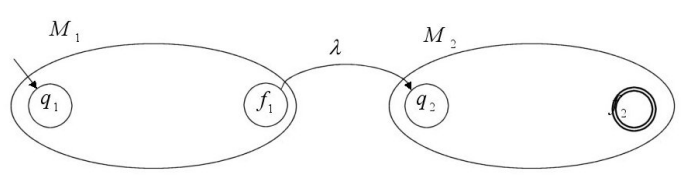
\includegraphics[scale=0.5]{imagenes/concat}
  \end{center}
\end{figure}

\paragraph{\(\bm{r_1^*}\):} \(M_0=\langle Q_0, \Sigma_1, \delta_0, q_0, \{f_0\}\rangle\):

\begin{itemize}
  \item \(Q_0 = Q_1 \cup \{f_0, q_0\}\)\
  \item \(\delta_1: Q_0 \times \Sigma_1 \rightarrow \mathcal{P}(Q_0)\)
        \begin{itemize}
          \item[] \(\delta(q_0, \lambda) = \delta(f_1,\lambda) = \{q_1, f_0\}\)
          \item[] \(\delta(q, a) = \delta_1(q, a)\) para \(q\in Q_1-\{f_1\}\) y \(a\in \Sigma_1\cup\{\lambda\}\)
        \end{itemize}
\end{itemize}
\begin{figure}[H]
  \begin{center}
    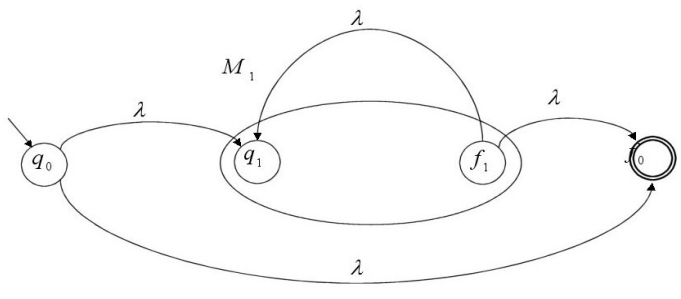
\includegraphics[scale=0.5]{imagenes/estrella}
  \end{center}
\end{figure}

Para el caso \(r_1^+\) es el mismo autómata que para este caso sin la transición \(q_0\overset{\lambda}{\rightarrow}f_0\).

\subsection{AFD a expresión regular}
\label{subsec:afd-er}
Dado un AFD \(M=\langle\{q_1, \dots, q_n\}, \Sigma, \delta, q_1, F\rangle\), que acepta el lenguaje \(\mathcal{L}\), existe una expresión regular que denota el mismo lenguaje.

\subsubsection{Demostración}
Nombremos \(R^k_{i,j}\) a la expresión regular cuyo lenguaje \(\omega \subseteq\Sigma^*\) son las cadenas que llevan al autómata \(M\) desde el estado \(q_i\) al estado \(q_j\) pasando solo por estados \(q_l\) con \(l\leq k\). En particular \(R^n_{i,j}\) es la expresión regular que representa todas las cadenas que permiten ir del estado \(i\) al estado \(j\).

Vamos a buscar como construir \(R^k_{i,j}\) para cada \(k\in\{0, \dots, n\}\) de manera inductiva. Suponiendo que demostramos la existencia de esta expresión regular, podemos concluir que la unión \(R^n_{1,f_1}|R^n_{1,f_2}|...|R^n_{1,f_m}\) (con \(f_1\dots f_m\in F\)) es la expresión regular que representa el lenguaje \(\mathcal{L}\):

\paragraph*{Caso base (\(k=0\)):} Como todos los estados están enumerados del 1 para arriba, \(k=0\) significa que no debe haber estados intermedios en el camino entre \(q_i\) y \(q_j\), por lo que pueden ser de dos formas:
\begin{itemize}
  \item Una arco del estado \(i\) al estado \(j\).
  \item Un camino de longitud cero que solo contiene el estado \(i\).
\end{itemize}

Si \(i\neq j\), entonces solo es posible la primera opción. Debemos examinar el AFD y encontrar aquellos simbolos que nos permitan ir del estado \(i\) al estado \(j\).

\begin{enumerate}
  \item Si no existe tal símbolo, entonces \(R^0_{i,j} = \varnothing\).
  \item Si existe exactamente un símbolo \(a\), entonces \(R^0_{i,j} = a\).
  \item Si existen más de un símbolo, entonces \(R^0_{i,j} = a_1|a_2|...|a_n\).
\end{enumerate}

Ahora, si \(i = j\) entonces los caminos de longitud cero también son posibles, por lo que habría que agregar a cada una de las expresiones recién mencionadas el simbolo \(\lambda\):
\begin{enumerate}
  \item \(R^0_{i,j} = \lambda\).
  \item \(R^0_{i,j} = a|\lambda\).
  \item \(R^0_{i,j} = a_1|a_2|...|a_n|\lambda\).
\end{enumerate}

\paragraph{Paso inductivo:} Supongamos que hay un camino desde el estado \(i\) al estado \(j\) que no pasa por estados mas grandes \(k\). Entonces podemos considerar las siguientes dos opciones:
\begin{enumerate}
  \item El camino no pasa por el estado \(k\), por lo que el lenguaje de \(R^{k-1}_{i,j}\) contiene a ese camino.
  \item El camino pasa por el estado \(k\) por lo menos una vez. Entonces podemos partir el camino en varias partes:
        \begin{figure}[H]
          \begin{center}
            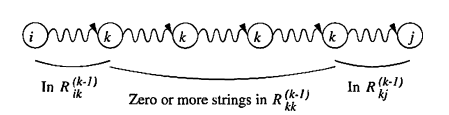
\includegraphics[scale=0.75]{imagenes/afd_regular.png}
          \end{center}
        \end{figure}
        La primer parte, va desde el estado \(i\) al estado \(k\) sin pasar por \(k\), la última parte es desde el estado \(k\) al estado \(j\) sin pasar por \(k\), y todas las partes intermedia s van desde el estado \(k\) al estado \(k\) sin pasar por \(k\). Cada una de estas partes ya tiene una expresión regular asociada: \(R^{k-1}_{i,k}\), \(R^{k-1}_{k,k}\), \(R^{k-1}_{k,j}\), por lo que podemos unirlas para obtener la expresión regular que representa el camino completo de la siguiente forma:
        \[
          R^{k-1}_{i,k}\left(R^{k-1}_{k,k}\right)^*R^{k-1}_{k,j}
        \]
\end{enumerate}

Entonces \(R^k_{i,j}\) es la unión de las expresiones de los dos tipos de caminos que acabamos de describir:
\[
  R^k_{i,j} = R^{k-1}_{i,j} \cup R^{k-1}_{i,k}\left(R^{k-1}_{k,k}\right)^*R^{k-1}_{k,j}
\]

Finalmente, si construimos en orden todas estas expresiones regulares desde \(R^0_{i,j}\), eventualmente llegaremos hasta \(R^n_{i,j}\).

Y como dijimos, más arriba si calculamos \(R^0_{1,j}\) para cada \(q_j\in F\) y unimos todas las expresiones, obtendremos la expresión regular que representa el lenguaje \(\mathcal{L}\).

\newpage
\subsection{Gramática regular a AFND}
Dada una grámatica regular \(G = \langle V_N, V_T, P, S\rangle\), podemos construir un AFND \(M=\langle Q,\Sigma, \delta, q_0, F\rangle\) que reconozca el lenguaje generado por \(G\)

\subsubsection{Demostración}
Vamos a constuir el autómata finito no determinista \(M\) y demostrar que reconoce el lenguaje generado por \(G\).
\paragraph{Construcción de \(M\):} Construyamos \(M\) de la siguiente manera:
\begin{itemize}
  \item \(Q = V_N\cup\{q_f\}\)
  \item \(\Sigma = V_T\)
  \item \(q_0 = q_S\)
  \item Si \(A, B \in V_N\) y \(a\in\Sigma\), entonces:
        \begin{itemize}
          \item \(q_B\in\delta(q_A, a) \iff A \rightarrow aB \in P\)
          \item \(q_f \in \delta(q_A, a) \iff A \rightarrow a \in P\)
          \item \(q_A\in F \iff A \rightarrow \lambda \in P\)
          \item \(q_f\in F\)
        \end{itemize}
\end{itemize}

\paragraph{Equivalencia clausura transitiva de producciones y \(\delta\): } Vamos a probar por inducción que
\[A   \overset{*}{\Rightarrow} \alpha B \iff q_B\in\hat\delta(q_A, \alpha)\]

\begin{itemize}
  \item \textbf{Caso base \(\alpha = \lambda\):}
        \begin{itemize}
          \item \(A\overset{*}{\Rightarrow} \alpha B\), pero las gramáticas regulares no acentan producciones que vayan de un no terminal a otro sin pasar por un terminal, por lo que \(B = A\). Osea \(A\overset{*}{\Rightarrow} \alpha A\).
          \item Además, como es un AFND, no tiene transiciones lambda, osea que \(\delta(q_A, \lambda) = \{q_A\}\), por lo que \(q_A\in\hat\delta(q_A, \alpha)\).
        \end{itemize}
  \item \textbf{Caso inductivo \(\alpha = \beta a\):}
        \begin{align*}
           & A\overset{*}{\Rightarrow} \alpha B  \iff A\overset{*}{\Rightarrow} \beta aB \underbrace{\iff}_{\text{def.}} \exists C\in V_N: A \overset{*}{\Rightarrow} \beta C \wedge C\rightarrow aB \\
           & \underbrace{\iff}_{\text{H.I. y def } M} \exists q_C\in Q, q_c\in\hat\delta(q_A,\alpha) \land q_B\in\delta(q_C,a) \iff q_B\in \delta(\hat\delta(q_A,\alpha),a)                          \\
           & \iff q_B\in\hat\delta(q_A, \beta a) \iff q_B\in\hat\delta(q_A, \alpha)                                                                                                                  \\
        \end{align*}
\end{itemize}

\paragraph{Demostración de la equivalencia:} Vamos a demostrar que el lenguaje generado por \(G\) y \(M\) son iguales, osea que \(\alpha a\in\mathcal{L}(M)\iff S\overset{*}{\Rightarrow} \alpha a\)
Como \(G\) es una grámatica regular, hay solo dos formas de llegar desde \(S\) hasta \(\alpha a\):
\begin{enumerate}
  \item \(\exists A\in V_N: S \overset{*}{\Rightarrow} \alpha A \wedge A \rightarrow a \in P\)
  \item \(\exists B\in V_N: S \overset{*}{\Rightarrow} \alpha aB \wedge B \rightarrow \lambda \in P\)
\end{enumerate}
Entonces:

\begin{align*}
   & S\overset{*}{\Rightarrow} \alpha a                                                                                                                                                                                                    \\
   & \underbrace{\iff}_{\text{def. gramatica regular}} (\exists A\in V_N: S \overset{*}{\Rightarrow} \alpha A \wedge A \rightarrow a \in P)\lor(\exists B\in V_N: S \overset{*}{\Rightarrow} \alpha aB \wedge B \rightarrow \lambda \in P) \\
   & \underbrace{\iff}_{\text{Equiv. anterior}} (\exists q_A\in Q, q_A\in\hat\delta(q_0, \alpha) \land q_f\in\delta(q_A, a)) \lor (\exists q_B\in Q, q_B\in\hat\delta(q_0, \alpha a) \land q_B\in F)                                       \\
   & \underbrace{\iff}_{\text{def. }\delta} q_f\in\delta(q_S, \alpha a) \lor (\exists q_B\in Q, q_B\in\hat\delta(q_0, \alpha a) \land q_B\in F)                                                                                            \\
   & \iff \alpha a \in \mathcal{L}(M)                                                                                                                                                                                                      \\
\end{align*}

Falta ver que pasa si \(\lambda\in\mathcal{L}(G)\):

\[ \lambda\in\mathcal{L}(G) \iff S\overset{*}{\Rightarrow} \lambda \iff S\rightarrow \lambda \in P \iff q_S\in F \iff \lambda \in \mathcal{L}(M)\]
\subsection{AFD a gramática regular}
Dado un AFD \(M=\langle Q, \Sigma, \delta, q_0, F\rangle\), existe una gramática regular \(G=\langle V_N, V_T, P, S\rangle\) equivalente

\subsubsection{Demonstración}
\paragraph{Contrucción de \(G\):} Vamos a construir \(G\) de la siguiente forma:
\begin{itemize}
  \item \(V_N = Q\), para mayor claridad llamamos \(A_p\) al no terminal correspondiente al estado \(p\in Q\)
  \item \(V_T = \Sigma\)
  \item \(S = q_0\)
  \item Si \(q\in Q \land q\notin F\) entonces \(A_p \rightarrow aA_q \in P \iff \delta(p,a) = q\)
  \item Si \(q\in F\) entonces \(A_p \rightarrow a \in P \iff \delta(p,a) = q\)
  \item \(S\rightarrow \lambda \in P \iff q_0\in F\)
\end{itemize}

\paragraph{Paso intermedio:} Vamos a demostrar por inducción: \[ \hat\delta(p,\alpha) = q \iff A_p \overset{*}{\Rightarrow} \alpha A_q\]

\begin{itemize}
  \item \textbf{Caso base:} \(\alpha = \lambda\) es trivial:
        \begin{align*}
           & \hat\delta(p,\lambda) = q \iff A_p \overset{*}{\Rightarrow} A_p
        \end{align*}
  \item \textbf{Caso inductivo \(\alpha = \beta a\):} Queremos probar que \(\hat\delta(p,\alpha) = q \iff A_p \overset{*}{\Rightarrow} \alpha A_q\).

        Nuestra hipotesis inductiva: \(\hat\delta(p,\beta) = q \iff A_p \overset{*}{\Rightarrow} \beta A_q\) para todo \(|\beta| \leq n\)

        \begin{align*}
           & \hat\delta(p, \alpha) = \hat\delta(p, \beta a) = q \underset{\text{def.}}{\iff}\exists r\in Q:~\hat\delta(p,\beta) = r \land \delta(r, a) = q                                                     \\
           & \iff\underbrace{\exists A_r, A_p \overset{*}{\Rightarrow} \beta A_r}_{\text{H.I}} \land \underbrace{A_r \rightarrow a A_q \in P}_{\text{constr. }G} \iff A_p \overset{*}{\Rightarrow} \beta a A_q \\
        \end{align*}
\end{itemize}

\paragraph{Demostración de equivalencia de lenguajes:}
\begin{align*}
   & \alpha a\in\mathcal{L}(M) \underset{\iff}{\text{def.}} \hat\delta(q_0, \alpha a) \in F \underset{\iff}{\text{def.}} \exists q\in Q:~\hat\delta(q_0, \alpha) = q \land \delta(q,a)\in F \\
   & \underset{\text{paso intermedio}}{\iff} \exists A_p, A_{q0} \overset{*}{\Rightarrow} \alpha A_p \land A_p \rightarrow a \in P \iff A_{q0} \overset{*}{\Rightarrow} \alpha a            \\
   & \underset{\text{def.}}{\iff} \alpha a \in\mathcal{L}(G)
\end{align*}

\newpage
\section{Minimización de AFD}
\subsection{Indistinguibilidad}
Sea \(M=\langle Q, \Sigma, \delta, q_0, F\rangle\) un AFD, decimos que \(p,q\in Q\),  son indistinguibles \((p\equiv q)\) si para toda cadena \(\alpha\in\Sigma^*\) tal que \(\hat\delta(p,\alpha) \in F\) entonces pasa que \(\hat\delta(q,\alpha) \in F\) y viceversa. Si \(p, q\in Q\) son indistinguibles, entonces decimos que \(p\) y \(q\) son equivalentes.

\[ p \equiv q \iff \forall \alpha \in \Sigma^*:~(\hat\delta(p,\alpha) \in F \iff \hat\delta(q,\alpha) \in F)\]

\paragraph{Teorema:} Si \(p\) y \(q\) son indistinguibles, sea \(\alpha\in\Sigma^*\) entonces \(\hat\delta(p,\alpha) \equiv \hat\delta(q,\alpha)\)

\[ p \equiv q \implies \forall \alpha \in \Sigma^*:~\hat\delta(p,\alpha) \equiv \hat\delta(q,\alpha)\]
\begin{demo}
  Sean \(p,q\in Q\), \(p\equiv q\).

  Supogamos que existe \(\alpha\in\Sigma^*\) tal que \(\hat\delta(p, \alpha) \not\equiv \hat\delta(q,\alpha)\) entonces existe una cadena \(\gamma\in\Sigma^*\) que distingue a \(\hat\delta(p,\alpha)\) de \(\hat\delta(q,\alpha)\). Osea que \(\hat\delta(\hat\delta(p,\alpha), \gamma) \in F\) y \(\hat\delta(\hat\delta(q,\alpha), \gamma) \not\in F\) (o viceversa).

  Por def: \(\hat\delta(\hat\delta(p,\alpha),\gamma) = \hat\delta(p,\alpha\gamma)\) y \(\hat\delta(\hat\delta(q,\alpha), \gamma) = \hat\delta(p,\alpha\gamma)\). Entonces, como \(\alpha\gamma\) es una cadena que nos permite distinguir \(p\) de \(q\), es decir \(p \not\equiv q\). Absurdo.
\end{demo}

\paragraph{Teorema:} \(\equiv\) es una relación de equivalencia.

\begin{demo}
  \begin{itemize}
    \item \textbf{Reflexividad:} \(p\equiv p\):
          \[ \forall \alpha \in \Sigma^*:~(\hat\delta(p,\alpha) \in F \iff \hat\delta(p,\alpha) \in F) \iff p \equiv p \]
    \item \textbf{Simetría:} \(p\equiv q \implies q\equiv p\):
          \begin{align*}
             & p \equiv q \implies \forall \alpha \in \Sigma^*:~(\hat\delta(p,\alpha) \in F \iff \hat\delta(q,\alpha) \in F)  \\
             & \iff \forall \alpha \in \Sigma^*:~(\hat\delta(q,\alpha) \in F \iff \hat\delta(p,\alpha) \in F) \iff q \equiv p
          \end{align*}
    \item \textbf{Transitividad:} \(p\equiv q \land q\equiv r \implies p\equiv r\):
          \begin{itemize}
            \item[] \(p \equiv q \implies \forall \alpha \in \Sigma^*:~(\hat\delta(p,\alpha) \in F \iff \hat\delta(q,\alpha) \in F)\)
            \item[] \(q \equiv r \implies \forall \alpha \in \Sigma^*:~(\hat\delta(q,\alpha) \in F \iff \hat\delta(r,\alpha) \in F)\)
          \end{itemize}
          Entonces
          \begin{align*}
             & \forall \alpha \in \Sigma^*:~(\hat\delta(p,\alpha) \in F \iff \hat\delta(r,\alpha) \in F) \iff p \equiv r
          \end{align*}
  \end{itemize}
\end{demo}
\end{document}